\documentclass[brazil]{beamer}
\usepackage[T1]{fontenc}
\usepackage[utf8]{inputenc}
\usepackage{lmodern}
\usepackage[brazilian]{babel}
\usetheme{JuanLesPins}

\title{Implementações de Runge-Kutta em C, CUDA e OpenCL}
\author{Giancarlo Rigo (gian.rigo@gmail.com) \\
        Rafael Reggiani Manzo (rr.manzo@gmail.com)}

\begin{document}
\maketitle

\section{Motivação}
\begin{frame}
  \frametitle{Motivação}
  
  \begin{itemize}
    \item Aplicações para visualização de imagens de tensores difusos (\textit{DTI - Diffusal Tensors Images}) costumam oferecer uma funcionalidade chamada de tractografia (\textit{fiber tracking}).
    \item Uma das formas de oferecer esta funcionalidade é com o algoritmo de Runge-Kutta para aproximação de problemas de valor inicial (\textit{IVP - Initial Value Problem}).
    \item Mas este algotimo é computacionalmente custoso na CPU. O que torna impossível sua implementação em tempo real.
    \item Para tonar possível os cálculos em tempo real implementações em GPU são uma solução já utilizada. 
  \end{itemize}
  
\end{frame}

\section{Runge-Kutta}
\begin{frame}
  \frametitle{Método de Runge-Kutta}
  
  \begin{itemize}
    \item O algoritmo é uma generalização do método de Euler para aproximação de solução de EDOs usando séries de Taylor
    \item Para o nosso caso vamos nos focar no método de ordem 2 (RK2) e  ordem 4 (RK4):
  \end{itemize}
 
  $ k_{1} = h\ldotp f(x_{n},y_{n}) $\\
  $ k_{2} = h\ldotp f(x_{n} + \frac{h}{2},y_{n} + \frac{k_{1}}{2}) $\\
  $ k_{3} = h\ldotp f(x_{n} + \frac{h}{2},y_{n} + \frac{k_{2}}{2}) $\\
  $ k_{4} = h\ldotp f(x_{n} + h,y_{n} + k_{3}) $\\
  $ y_{n+1} = y_{n} + \frac{k_{1}}{6} + \frac{k_{2}}{3} + \frac{k_{3}}{3} + \frac{k_{4}}{6} + O(h^{5}) $ 
  
\end{frame}

\subsection{Adapatação a campos vetoriais}
\begin{frame}
  \frametitle{Problemas para campos vetoriais}
  
  \begin{itemize}
    \item Em campos vetoriais não temos EDOs.
    \item Campos vetoriais são discretos e no caso de \textit{DTI} nem todos os pontos possuem um vetor associado.
  \end{itemize}
\end{frame}

\begin{frame}
  \frametitle{Soluções}
  \framesubtitle{Quanto as EDOs}
  
  \begin{itemize}
    \item Temos vetores que podemos interpretar como a direção da reta tangente na direção da função que desejamos aproximar.
    \item O que nos leva a seguinte expressão para o RK4:
  \end{itemize}

  $k_{1} = h\ldotp (\alpha ,\beta ,\gamma )$\\
  $k_{2} = \frac{k_{1}}{2} + h\ldotp (\alpha ,\beta ,\gamma )$\\
  $k_{3} = \frac{k_{2}}{2} + h\ldotp (\alpha ,\beta ,\gamma )$\\
  $k_{4} = k_{3} + h\ldotp (\alpha ,\beta ,\gamma )$\\
  $(x_{n+1}, y_{n+1}, z_{n+1}) = (x_{n}, y_{n}, z_{n}) + \frac{k_{1}}{6} + \frac{k_{2}}{3} + \frac{k_{3}}{3} + \frac{k_{4}}{6}$

\end{frame}

\begin{frame}
  \frametitle{Soluções}
  \framesubtitle{Quanto a natureza discreta do campo}

  \begin{itemize}
    \item Em pontos nos quais não há um vetor associado, fazemos a interpolação (\textit{Trilinear interpolation}).
    \item No limite do campo não teremos todos os pontos necessários para a interpolação. Então usamos o mais simples possível que é buscar o vizinho mais próximo (\textit{Nearest Neighbour}).
  \end{itemize}
\end{frame}

\section{Implementação}

\begin{frame}
  \frametitle{Problema que desejamos resolver}
  \begin{itemize}
    \item Muitas vezes queremos calcular as fibras (equivalente à função) que passam por vários pontos iniciais diferentes e nos sentidos positivo e negativo. Tudo isso ao mesmo tempo.
    \item Ou seja, temos que aplicar o mesmo método repetidamente uma quantidade muito grande de vezes para fazer isto em tempo real.
  \end{itemize}
\end{frame}

\begin{frame}
  \frametitle{Paralelizável}
  
  \begin{itemize}
    \item Cada ponto inicial e cada direção são instâncias independentes (o ponto de uma fibra, idealmente, não é influenciado por outra fibra) do problema que podem ser resolvidas concorrentemente.
    \item Então temos um problema altamente paralelizável que envolve múltiplas operações de ponto flutuante.
  \end{itemize}
\end{frame}


\subsection{GPGPU}
\begin{frame}
  \frametitle{GPGPU}
  \framesubtitle{General Purpose Computing on Graphics Processing Units}
  
  Computação de propósito geral na unidade de processamento gráfico.
  
  \begin{itemize}
    \item As GPUs são utilizadas principalmente para processamento gráfico, mas descobriu-se seu poder de processamento é muito interessante também para outros tipos de processamento que envolvam cálculos e sejam altamente paralelizáveis.
    \item Uma NVIDIA GeForce GTX 690 possui mais de 3000 núcleos de processamento (\textit{CUDA Cores}) a aproximadamente 900MHz cada e 4GB de memória dedicada.
  \end{itemize}
  
  Então este é um ambiente bastante propenso para implementarmos nosso algoritmo e obtermos a tractografia em tempo real.
\end{frame}

\begin{frame}
  \frametitle{Implementação de algoritmos gerais em GPU}
  \begin{itemize}
    \item No inicío era feito em termos de operações gráficas (produto de matrizes de textura por exemplo)
    \item Com o surgimento da linguagem Cg isso se tornou mais plausível, mas ela ainda é uma linguagem baseada no C que é convertida em termos de DirectX ou shaders do OpenGL.
    \item Percebendo a necessidade de algo mais próximo às linguagens de propósito geral, surgiram outras duas linguagens CUDA e OpenCL que podem ser utilizadas como extensões das linguagens C, C++ e Fortran.
  \end{itemize}
\end{frame}

\begin{frame}
  \frametitle{Comparação teórica}

\begin{columns}
  \begin{column}{.5\textwidth}
    CUDA
    
    \begin{itemize}
      \item Propriedade da NVIDIA.
      \item Apenas para GPUs NVIDIA (apesar de seguir o padrão LLVM, só existe compilador para GPUs NVIDIA).
      \item Alto acoplamento ao código (é possível mesclar CUDA com outras linguagens no mesmo arquivo fonte).
      \item Tem maior conhecimento do hardware permitindo otimizações específicas para este.
    \end{itemize}
  \end{column}
  \begin{column}{.5\textwidth}
    OpenCL    
    
    \begin{itemize}
      \item A marca é propriedade da Apple (desenvolveu a primeira versão), mas desenvolvido atualmente como colaboração entre AMD, IBM, Intel e NVIDIA.
      \item Executado em GPUs e CPUs de qualquer fabricante desde que com os drivers apropriados.
      \item Obrigatoriamente o fonte OpenCL tem que estar separado do restante.
    \end{itemize}
  \end{column}
\end{columns}
\end{frame}

\begin{frame}
  \frametitle{Características importantes da arquitetura da GPU}
  
  \begin{itemize}
    \item O trecho de código executado na GPU é chamado de \textit{kernel}.
    \item Um mesmo \textit{kernel} é executado em múltiplas \textit{threads} que por sua vez podem estar separadas em múltiplos blocos (\textit{blocks}) que por sua vez podem estar em múltiplas grades (\textit{grids}).
    \item Os núcleos da GPU estão agrupados em SMs (\textit{stream multiprocessors}) cada um com uma memória compartilhada dedicada e 32 núcleos cada.
    \item Todas as threads de um bloco são necessariamente escalonadas para o mesmo SM.
    \item A GPU se encarrega do escalonamento. Sua menor unidade é um \textit{warp}, que corresponde a um conjunto de 16 \textit{threads}.
  \end{itemize}
\end{frame}

\subsection{Estado atual}
\begin{frame}
  \frametitle{O que foi feito}

  \begin{itemize}
    \item Implementações do RK2 e RK4 em C++, CUDA e OpenCL.
    \item Profiling para as implementações C++ e CUDA.
    \item Visualização do campo vetorial e do resultado do método em OpenGL.
    \item Resultado do método pode ser exportado para o GNUPlot.
  \end{itemize}
\end{frame}

\begin{frame}
  \frametitle{Visualização}
  \framesubtitle{GNUPlot}
  
    \begin{figure}
    \begin{center}
      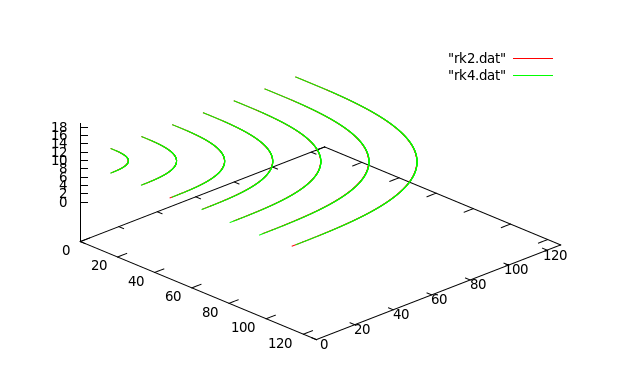
\includegraphics[width=80mm, height=50mm]{rk2-vs-rk4.png}
      \caption{Visualização no GNUPlot do resultado dos algoritmos para um campo vetorial 128x128x20 que representa uma rotação no eixo z.}
    \end{center}
  \end{figure}
\end{frame}

\begin{frame}
  \frametitle{Visualização}
  \framesubtitle{OpenGL}
  
    \begin{figure}
    \begin{center}
      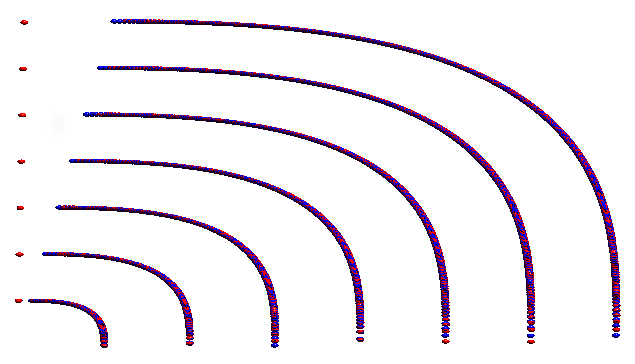
\includegraphics[width=80mm, height=50mm]{rk2-vs-rk4-opengl.png}
      \caption{Visualização no OpenGL do resultado dos algoritmos para um campo vetorial 128x128x20 que representa uma rotação no eixo z.}
    \end{center}
  \end{figure}
\end{frame}

\end{document}
